\section{Минимизация логической функции}

\subsection{Постановка задачи}

Требуется минимизировать логическую функцию, преставленную в дизъюнктивной нормальной форме 
и содержащую следующие конъюнктивные термы:

\begin{center}
    $ab\bar{c}$,
    $acd$,
    $b\bar{c}d$,
    $\bar{a}\bar{b}\bar{c}$,
    $\bar{a}\bar{b}cd$,
    $\bar{a}\bar{b}\bar{c}\bar{d}$,
    $abc\bar{d}$.
\end{center}

Минимизацию функции производить одним из следующих методов - Квайна или Карно.

\subsection{Описание алгоритма минимизации логической функции}

По условию задачи необходимо минимизировать логическую функцию 4-х переменных.
Для этого воспользуемся методом минимизирующих карт Карно.

\vspace{1em}

Алгоритм минимизации картами Карно состоит в следующем:

\begin{enumerate}
    \item Графически представить логическую функцию соответствующей ей картой Карно.

    \item Покрыть все минтермы наименьшим числом наибольших контуров, размеры которых кратны степени двойки.

    \item По постоянным переменным контура записать соответствующий ему элементарный конъюнкт.
    
    \item Из полученных элементарных конъюнктов составить минимальную нормальную дизъюнктивную форму (МДНФ).

    \item Конец алгоритма.
\end{enumerate}

\subsection{Переход от ДНФ к СДНФ}

Для построения таблицы истинности представим логическую функцию в совершенной нормальной дизъюнктивной форме (СДНФ):

\vspace{1em}

$F = ab\bar{c}(d\vee\bar{d})\vee acd(b\vee\bar{b})\vee b\bar{c}d(a\vee\bar{a})\vee\bar{a}\bar{b}\bar{c}(d\vee\bar{d})\vee\bar{a}\bar{b}cd\vee\bar{a}\bar{b}\bar{c}\bar{d}\vee abc\bar{d}
   = ab\bar{c}d\vee ab\bar{c}\bar{d}\vee abcd\vee a\bar{b}cd\vee ab\bar{c}d\vee\bar{a}b\bar{c}d\vee\bar{a}\bar{b}\bar{c}d\vee\bar{a}\bar{b}\bar{c}\bar{d}\vee\bar{a}\bar{b}cd\vee\bar{a}\bar{b}\bar{c}\bar{d}\vee abc\bar{d}
   = ab\bar{c}d\vee ab\bar{c}\bar{d}\vee abcd\vee a\bar{b}cd\vee\bar{a}b\bar{c}d\vee\bar{a}\bar{b}\bar{c}d\vee\bar{a}\bar{b}\bar{c}\bar{d}\vee\bar{a}\bar{b}cd\vee abc\bar{d}$.

\vspace{1em}

$F_{\mbox{\tiny СДНФ}}
= ab\bar{c}d\vee ab\bar{c}\bar{d}\vee abcd\vee a\bar{b}cd\vee\bar{a}b\bar{c}d\vee\bar{a}\bar{b}\bar{c}d\vee\bar{a}\bar{b}\bar{c}\bar{d}\vee\bar{a}\bar{b}cd\vee abc\bar{d}$.

\vspace{1em}

Полученное представление функции состоит из термов максимального ранга (минтермов). 

\subsection{Минимизация методом карт Карно}

На основании представления функции $F$ в виде СДНФ, построим минимизирующую карту
Карно для данной функции:

\begin{figure}[h!]
    \centering
    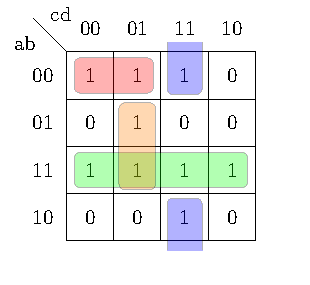
\includegraphics[scale=1.5]{S2IM1.pdf}  
    \caption{Карта Карно для функции F(a,b,c,d)}
    \label{fig:task2:karnaugh_map}
\end{figure}

На рисунке~\ref{fig:task2:karnaugh_map} изображена карта Карно с наименьшим числом наибольших покрытий минтермов.
На основании покрытий получим минимальную дизъюнктивную нормальную форму функции:

\begin{equation*}
    F_{\mbox{\tiny МДНФ}}
    = ab \vee \bar{a}\bar{b}\bar{c} \vee b\bar{c}d \vee \bar{b}cd. 
\end{equation*}